\documentclass{article}
\usepackage[utf8]{inputenc}
\usepackage[T1]{fontenc}
\usepackage[margin=1in]{geometry}
\usepackage{amsmath}
\usepackage{booktabs}
\usepackage[hidelinks]{hyperref}
\usepackage{natbib}
\usepackage{caption}
\usepackage{pgfplots}
\pgfplotsset{compat=1.17}
\usepgfplotslibrary{groupplots}
\usetikzlibrary{patterns,arrows.meta,positioning,fit,backgrounds,shapes.geometric,calc}

% Emit every tikzpicture as a standalone PDF in tikz-figures/ (needs -shell-escape).
\usetikzlibrary{external}
\tikzexternalize[prefix=tikz-figures/]

\captionsetup{font=small,labelfont=bf}

% ---- shared colours ----
\definecolor{cUnc}{HTML}{7F7F7F}
\definecolor{cCOMs}{HTML}{E1812C}
\definecolor{cGABO}{HTML}{9467BD}
\definecolor{cOurs}{HTML}{1F77B4}
\definecolor{cFM}{HTML}{1F77B4}
\definecolor{cSimple}{HTML}{7F7F7F}
\definecolor{cGFP}{HTML}{D9722B}
\definecolor{cRed}{HTML}{C0392B}
\definecolor{cBox}{HTML}{F2F4F7}
\definecolor{cBoxEdge}{HTML}{9AA5B1}
\definecolor{cFrozen}{HTML}{3B82C4}
\definecolor{cGate}{HTML}{1F77B4}
\definecolor{cBad}{HTML}{C0392B}
\definecolor{cGood}{HTML}{2E8B57}
\definecolor{cVal}{HTML}{7E57C2}

\title{\textbf{Attack-as-Design: Turning Surrogate Exploitation into
Validated Biological Sequence Design}}
\author{Ajay Rangarajan \and Jeyashree Krishnan}
\date{}

\begin{document}
\maketitle

\begin{abstract}
\noindent
The same search that produces \emph{adversarial examples}---driving a model's prediction up
by making small changes to its input---can be turned into a tool for designing biological
sequences. We train a small model to predict a property (the \emph{surrogate}) and then run
an attack-style search to find sequences the surrogate scores highly. On its own this search
cheats: it finds sequences that fool the surrogate into predicting a high score rather than
sequences that are genuinely good. We make the search useful by adding two things. First, a
simple biological rule that keeps every proposed sequence realistic, using no extra trained
model: each change from the starting sequence must be conservative under the BLOSUM62
(BLOcks SUbstitution Matrix) table, and a set of whole-sequence biophysical numbers
(hydrophobicity, net charge, aromatic and charged fractions, sequence complexity, and the
longest repeated-letter run) must stay within the ranges seen in natural sequences. Second,
and most important, we check every design against signals the search never used---so the
final claim never rests on the surrogate grading its own work. We demonstrate the system on
\textbf{four tasks across two molecule types}: protein thermostability and green fluorescent
protein (GFP) fluorescence, a 600-base-pair regulatory-DNA task verified on a true
functional model (Borzoi), and a small DNA benchmark with an exact ground-truth answer
(TF-Bind-8) used as a diagnostic. The biological rule keeps 100\% of GFP designs realistic
versus 5--19\% for the baselines (paired Wilcoxon $p<10^{-7}$); on thermostability it matches
a learned second model and beats a hand-tuned penalty ($p<0.001$); and on regulatory DNA the
system raises the true property on all 40 of 40 starting points. Independent checks (a
structure predictor, a separate thermostability predictor, kept functional residues, and a
true DNA-activity model) agree the designs are real. Which featurization the surrogate uses
(a frozen foundation-model embedding or a plain one-hot/$k$-mer encoding) is a swappable
part of the system, reported as an ablation, not the point: the foundation model only helps
on long, variable-length protein, and the system works either way.
\end{abstract}

\section{Introduction}

Many sequence design problems are posed as optimizing a measured property $y$ over
sequences $x$: find the DNA, RNA, or protein sequence that maximizes binding affinity,
thermostability, or activity. Because direct measurement is costly, a common approach is to
train a \emph{surrogate} model that predicts $y$ from $x$ using available measurements, and
then search for sequences the surrogate scores highly. This is the setting of offline
model-based optimization \citep{trabucco2021coms, trabucco2022designbench}.

This approach has a well-known weakness. A surrogate is only accurate near the sequences it
was trained on. When the search pushes into unusual sequences, the surrogate can assign them
a high score by mistake, and the search happily returns those mistakes instead of genuinely
good sequences. This is exactly the mechanism behind an ``adversarial example'' in image
classification, where a small, deliberately chosen change fools a model into a confident
wrong answer. The offline optimization literature already makes this connection
\citep{trabucco2021coms, trabucco2022designbench, fu2021nemo}; we build on it rather than
claim it.

Our starting observation is that this weakness is also an opportunity. The search that
exploits the surrogate is the \emph{same machinery} used to generate adversarial examples---a
population-based or gradient search that pushes a model's output up. If we can stop it from
walking off into unrealistic sequences, the same engine becomes a sequence \emph{designer}.
This is the paper's thesis: \textbf{attack-as-design}. What turns exploitation into design is
not a new search algorithm, but two additions---a rule that keeps the search realistic, and a
validation protocol that confirms the designs are real using signals the search never saw.

Existing ways to keep the search realistic add a trained component. One trains a second model
to tell training-like sequences from proposed ones, and uses it to lower the score of
sequences that look unfamiliar \citep{yao2024gabo}. Another adds a penalty that pushes the
surrogate to predict lower scores on the sequences the search proposes
\citep{trabucco2021coms}. Both work, and both add an extra piece that must itself be trained
or tuned. We ask whether a fixed biological rule, which trains nothing, does as well.

The surrogate itself can be built on a \emph{foundation model}: a network pre-trained on
large sequence corpora that maps a sequence to a fixed-length embedding
\citep{lin2023esm2, zhou2023dnabert2}, on top of which a lightweight predictor is trained.
We treat this as a swappable choice inside the system, not as the contribution: the
featurization can equally be a plain one-hot or $k$-mer encoding, and we report the
comparison as an ablation (Section~\ref{sec:experiments}).

\paragraph{Approach.}
We ask whether a rule that uses no extra trained model is enough. Our rule has two parts,
and neither one looks at the surrogate:
\begin{enumerate}
\item \textbf{Conservative substitutions.} Each substitution relative to the starting
sequence must be conservative under the BLOSUM62 (BLOcks SUbstitution Matrix) substitution
matrix \citep{henikoff1992blosum}, a standard table scoring how often one amino acid
replaces another in related natural proteins.
\item \textbf{Biophysical window.} Global sequence descriptors---mean hydrophobicity, net
charge per residue, aromatic and charged fractions, sequence complexity, and the longest
homopolymer run---must lie within the 1st--99th percentile range measured on the training
proteins.
\end{enumerate}
A candidate that breaks either part is thrown out during the search. We compare this rule
against a hand-tuned penalty (COMs, Conservative Objective Models) and a learned second
model (GABO/aSCR, Generative Adversarial Bayesian Optimization with an adaptive Source-Critic
Regularization). All methods use the same search algorithm, the same starting points, the
same budget, and the same evaluation; they differ only in how they keep the search realistic.

\paragraph{Contributions.}
(i) \textbf{The system works as a designer.} Attack-style search under the biological rule
raises the true property on three design tasks---protein thermostability, GFP fluorescence,
and 600-base-pair regulatory DNA (all 40 of 40 starting points improved on a true DNA-activity
model). (ii) \textbf{Every design is independently validated.} On each task the gain is
confirmed by a signal the search never used: a held-out predictor ensemble, a separate
model family (TemStaPro), a structure predictor (AlphaFold2), kept functional residues, and
an exact ground-truth oracle (TF-Bind-8). This surrogate-blind validation protocol is the
methodological contribution, not a new optimizer. (iii) \textbf{We characterize when the
rule helps and when it hurts.} The rule earns its keep only when the search is exploitable
and the realistic range is both narrow and aligned with the true objective; a poorly aligned
rule can even reduce the true property (we show this on a DNA task). (iv) \textbf{The
surrogate is swappable.} A frozen foundation-model embedding beats a plain encoding only on
long, variable-length protein; on short DNA a one-hot encoding wins. None of the system's
claims depend on this choice.

\begin{figure}[t]
\centering
\tikzsetnextfilename{overview}
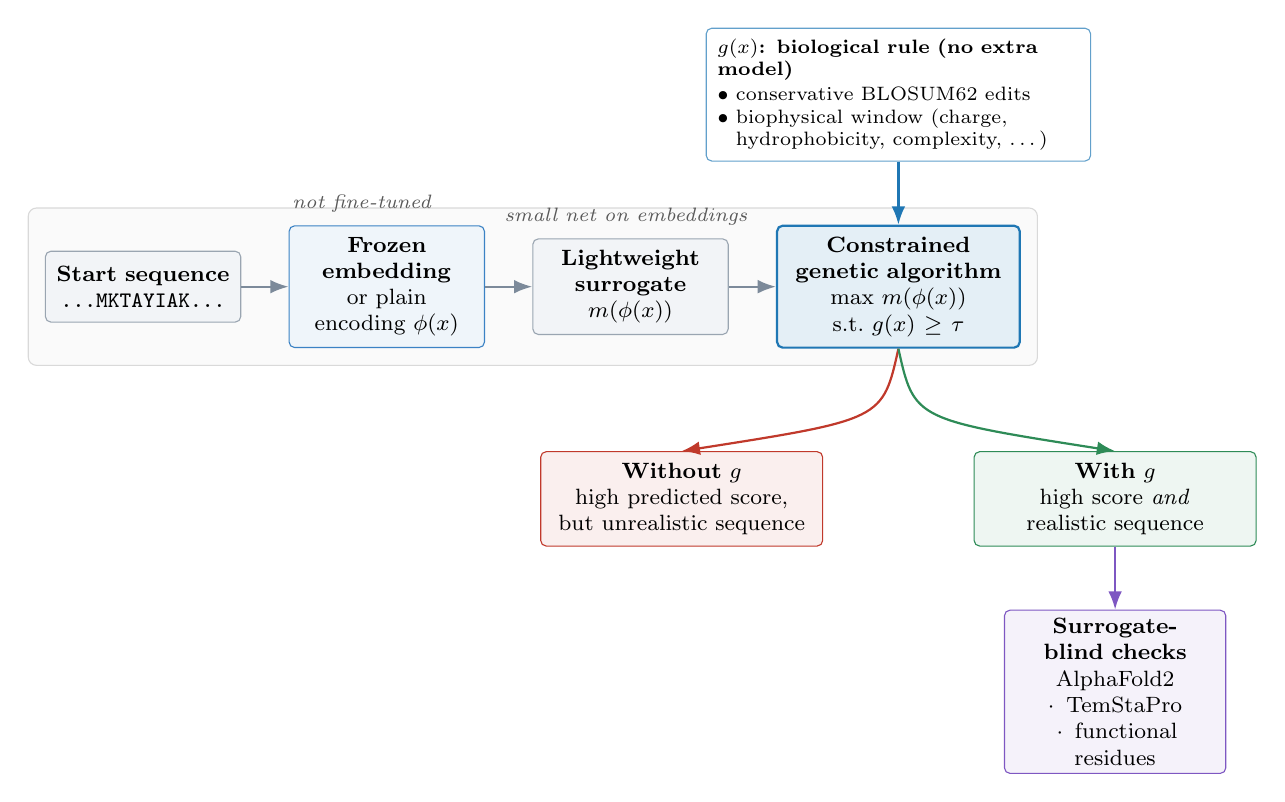
\begin{tikzpicture}[
  font=\footnotesize,
  >=Latex,
  node distance=6mm,
  box/.style={draw=cBoxEdge, fill=cBox, rounded corners=2pt, align=center,
              inner sep=4pt, minimum height=9mm, text width=22mm},
  frozen/.style={draw=cFrozen, fill=cFrozen!8, rounded corners=2pt, align=center,
              inner sep=4pt, minimum height=9mm, text width=22mm},
  gate/.style={draw=cGate, fill=cGate!12, rounded corners=2pt, align=center,
              inner sep=4pt, minimum height=9mm, text width=28mm, thick},
  outbad/.style={draw=cBad, fill=cBad!8, rounded corners=2pt, align=center,
              inner sep=4pt, minimum height=9mm, text width=33mm},
  outgood/.style={draw=cGood, fill=cGood!8, rounded corners=2pt, align=center,
              inner sep=4pt, minimum height=9mm, text width=33mm},
  val/.style={draw=cVal, fill=cVal!8, rounded corners=2pt, align=center,
              inner sep=3pt, minimum height=7mm, text width=26mm},
  flow/.style={->, thick, draw=cBoxEdge!130},
  lbl/.style={font=\scriptsize\itshape, text=black!65},
]
% ---- top row: the shared pipeline ----
\node[box] (seq) {\textbf{Start sequence}\\ \texttt{...MKTAYIAK...}};
\node[frozen, right=of seq] (emb) {\textbf{Frozen embedding}\\ or plain encoding $\phi(x)$};
\node[box, right=of emb] (sur) {\textbf{Lightweight}\\ \textbf{surrogate} $m(\phi(x))$};
\node[gate, right=of sur] (ga) {\textbf{Constrained}\\ \textbf{genetic algorithm}\\ $\max\, m(\phi(x))$ s.t.\ $g(x)\!\ge\!\tau$};

\draw[flow] (seq) -- (emb);
\draw[flow] (emb) -- (sur);
\draw[flow] (sur) -- (ga);

\node[lbl, above=1pt of emb, text width=24mm] {not fine-tuned};
\node[lbl, above=1pt of sur, text width=32mm] {small net on embeddings};

% ---- constraint annotation above the gate (keeps the outcome branch below it clear) ----
\node[draw=cGate!70, fill=white, rounded corners=2pt, above=8mm of ga,
      align=left, inner sep=4pt, text width=46mm, font=\scriptsize] (con)
  {\textbf{$g(x)$: biological rule (no extra model)}\\[1pt]
   $\bullet$ conservative BLOSUM62 edits\\
   $\bullet$ biophysical window (charge,\\ \phantom{$\bullet$ }hydrophobicity, complexity, \dots)};
\draw[->, thick, draw=cGate] (con) -- (ga);

% ---- two outcomes ----
\node[outbad, below left=13mm and -6mm of ga] (bad)
  {\textbf{Without $g$}\\ high predicted score,\\ but unrealistic sequence};
\node[outgood, below right=13mm and -6mm of ga] (good)
  {\textbf{With $g$}\\ high score \emph{and}\\ realistic sequence};

\draw[->, thick, draw=cBad] (ga.south) .. controls +(-0.2,-0.9) .. (bad.north);
\draw[->, thick, draw=cGood] (ga.south) .. controls +(0.2,-0.9) .. (good.north);

% ---- surrogate-blind validation ----
\node[val, below=8mm of good] (val)
  {\textbf{Surrogate-blind checks}\\ AlphaFold2 \,$\cdot$\, TemStaPro\\ \,$\cdot$\, functional residues};
\draw[->, thick, draw=cVal] (good) -- (val);

% grouping backdrop for the shared pipeline
\begin{scope}[on background layer]
  \node[draw=black!15, rounded corners=3pt, fit=(seq)(emb)(sur)(ga),
        inner sep=6pt, fill=black!2] {};
\end{scope}
\end{tikzpicture}
\caption{\textbf{Overview of the attack-as-design system.} A starting sequence is mapped to a
featurization (a frozen foundation-model embedding, or a plain one-hot/$k$-mer encoding---a
swappable choice); a small surrogate predicts the property; the same search used to generate
adversarial examples looks for sequences the surrogate scores highly, subject to a biological
rule $g(x)\ge\tau$ (conservative BLOSUM62 substitutions and a biophysical window) that uses no
extra model. Without the rule, the search finds sequences that score highly but are
unrealistic; with the rule, the sequences it returns are both high-scoring and realistic.
Every design is then checked by signals the search never used---the load-bearing step.}
\label{fig:overview}
\end{figure}

\section{Method}

Figure~\ref{fig:overview} summarizes the pipeline. Its components are described below.

\paragraph{Surrogate.}
The surrogate maps a sequence $x$ to a featurization $\phi(x)$ and then predicts the
property with a small neural network $m$ (a multilayer perceptron, MLP). For the protein
tasks $\phi$ is a frozen ESM-2 (Evolutionary Scale Modeling, version 2)
\citep{lin2023esm2} embedding: we run the foundation model,
average its per-residue outputs into one fixed-length vector, and never update the model
itself. The featurization is a swappable choice---$\phi$ can equally be a one-hot or
$k$-mer encoding---and we treat the comparison as an ablation
(Section~\ref{sec:experiments}), not as part of the system's claims.

\paragraph{Optimizer and objective.}
We search with a genetic algorithm (GA), a population-based search that maintains a set of
candidates, scores them with the surrogate, retains the highest-scoring individuals, and
generates new candidates from them by changing one residue at a time. Run without any rule,
this is exactly the search that tends to find the surrogate's mistakes. We solve
\[
\max_{x}\; m\big(\phi(x)\big) \quad \text{subject to}\quad g(x) \ge \tau,
\]
where $g(x)\ge\tau$ is the biological rule. The compared methods differ only in $g$; the
embedding, the search, the starting sequences, the budget, and the evaluation are the same
for all of them.

\paragraph{Compared methods.}
\emph{Unconstrained} just maximizes the surrogate, with no rule. \emph{COMs}
\citep{trabucco2021coms} adds a penalty that trains the surrogate to give lower scores to
the sequences the search proposes; we tuned its strength for a fair comparison.
\emph{GABO/aSCR} \citep{yao2024gabo} trains a second model that scores how far a sequence is
from the training data, and uses it to discount unfamiliar designs. \emph{Ours} applies the
biological rule (conservative BLOSUM62 substitutions and the biophysical window), which
trains nothing extra.

\paragraph{Evaluation.}
We never let the surrogate grade its own designs. We report: (i) \emph{real gain}, measured
by a separate set of predictor models that the search never used; (ii)
\emph{naturalness} ($\Delta$PLL), the change in the foundation model's masked language-model
pseudo-log-likelihood (PLL), a score of how expected a sequence is under the model, where
higher values indicate greater naturalness;
(iii) \emph{biophysical pass rate}, the fraction of designs within the natural descriptor
range; and (iv) for a subset, three fully independent measures: AlphaFold2
\citep{jumper2021alphafold, mirdita2022colabfold} predicted local distance difference test
(pLDDT), the independent thermostability predictor TemStaPro
\citep{pudziuvelyte2024temstapro}, and preservation of known functional residues.

\section{Experiments}
\label{sec:experiments}

We evaluate the system on four public tasks across two molecule types. Two are protein
design tasks. \textbf{Meltome} provides melting temperatures for approximately 28{,}000
proteins from the FLIP (Fitness Landscape Inference for Proteins) benchmark
\citep{dallago2021flip, jarzab2020meltome}. \textbf{GFP} provides fluorescence for
approximately 52{,}000 variants of a single 238-residue green fluorescent protein from
ProteinGym \citep{notin2023proteingym, sarkisyan2016gfp}. Their surrogates predict the
property from frozen ESM-2 embeddings with rank correlation $\rho\approx0.67$ (Meltome) and
$\rho\approx0.80$ (GFP). Two are DNA tasks. \textbf{Regulatory DNA} designs 600-base-pair
sequences for chromatin accessibility, verified on Borzoi \citep{linder2025borzoi}, a
published model of DNA activity used here as a true functional oracle. \textbf{TF-Bind-8}
\citep{barrera2016tfbind, trabucco2022designbench} lists all $65{,}536$ 8-letter DNA
sequences with their measured transcription-factor binding, giving an exact ground-truth
answer for every sequence; we use it as a diagnostic. For each design task we optimize 40
mid-range starting sequences under a shared query budget. The biological rule is adapted to
the molecule type: BLOSUM62 substitutions plus the biophysical window for proteins, and a
composition band (GC content, repeated-letter cap, and $k$-mer diversity) derived from the
training sequences for DNA.

The core results are the design head-to-heads (Meltome, GFP) and the regulatory-DNA design
task, each with independent validation. Two further results scope the system: an ablation on
the surrogate featurization, and a diagnostic on the exact TF-Bind-8 oracle. We present the
scoping results first because they set up how the design results should be read.

\subsection{Ablation: when is a foundation model needed?}

The surrogate's featurization is a swappable part of the system. Here we ask when it matters.
We compare frozen-embedding surrogates against trivial encodings (a one-hot encoding
records each position's letter directly; a $k$-mer count records how often each short
subsequence appears) across four tasks of increasing input length (Table~\ref{tab:decode},
Figure~\ref{fig:decode}). The two short-DNA tasks (TF-Bind-8) measure how strongly a
transcription factor binds each 8-base-pair DNA sequence. On 8-base-pair DNA, a one-hot
encoding attains higher rank
correlation than the DNA foundation model; on 300-base-pair DNA the two are comparable.
The foundation model only helps clearly for proteins, whose variable length means a simple
encoding cannot be used. This tells us when the method is worth using: on long,
variable-length sequences where simple encodings run out.

\begin{table}[t]
\centering\small
\caption{Held-out rank correlation (Spearman $\rho$) of the property from a frozen
foundation-model (FM) embedding versus a trivial encoding, across four tasks.}
\label{tab:decode}
\begin{tabular}{llrlrl}
\toprule
Task & Input & FM $\rho$ & Simple encoding & Simple $\rho$ & Higher \\
\midrule
TF-Bind-8 (SIX6) & 8 bp DNA & 0.53 & one-hot & 0.77 & simple \\
TF-Bind-8 (WT1)  & 8 bp DNA & 0.71 & one-hot & 0.87 & simple \\
Promoter (EPDnew) & 300 bp DNA & 0.28 & 4-mer counts & 0.29 & comparable \\
Meltome (FLIP) & $\sim$400 aa protein & 0.67 & amino-acid composition & 0.50 & FM \\
\bottomrule
\end{tabular}
\end{table}

\begin{figure}[t]
\centering
\tikzsetnextfilename{decode}
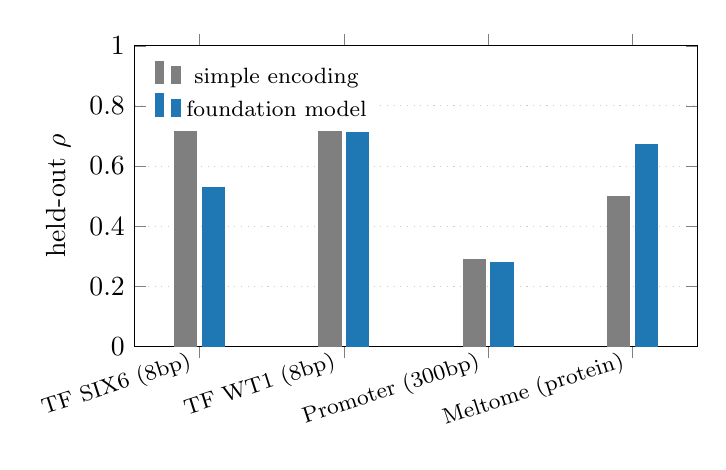
\begin{tikzpicture}
\begin{axis}[
  width=0.72\textwidth, height=5.4cm,
  ybar, bar width=8pt,
  ymin=0, ymax=1,
  ylabel={held-out $\rho$},
  symbolic x coords={TF SIX6 (8bp), TF WT1 (8bp), Promoter (300bp), Meltome (protein)},
  xtick=data, x tick label style={rotate=18, anchor=east, font=\footnotesize},
  ytick={0,0.2,0.4,0.6,0.8,1.0},
  legend style={at={(0.02,0.97)}, anchor=north west, font=\footnotesize, draw=none},
  enlarge x limits=0.15, ymajorgrids, major grid style={dotted,gray!40},
]
\addplot[fill=cSimple,draw=cSimple] coordinates
 {(TF SIX6 (8bp),0.77) (TF WT1 (8bp),0.87) (Promoter (300bp),0.29) (Meltome (protein),0.50)};
\addplot[fill=cFM,draw=cFM] coordinates
 {(TF SIX6 (8bp),0.53) (TF WT1 (8bp),0.71) (Promoter (300bp),0.28) (Meltome (protein),0.67)};
\legend{simple encoding, foundation model}
\end{axis}
\end{tikzpicture}
\caption{\textbf{When is a foundation model needed?} A surrogate on frozen foundation-model
embeddings (blue) beats a simple encoding (grey) only for variable-length proteins. On short
DNA the simple encoding is stronger; on 300-bp DNA the two are about the same.}
\label{fig:decode}
\end{figure}

\subsection{A small DNA benchmark, used as a diagnostic}

The TF-Bind-8 benchmark \citep{barrera2016tfbind, trabucco2022designbench} lists all
$65{,}536$ possible 8-letter DNA sequences together with their measured binding, so the true
answer is known for every sequence. On this benchmark every method reaches about the same
true score for its best designs, including plain random search ($\approx0.89$): the space is
simply too small for the methods to pull apart on performance. What they do differ on is how
much the surrogate overrates its own designs---the gap between the score the surrogate
predicts and the true score (Figure~\ref{fig:tfbind}). Gradient ascent and AdaLead (a
greedy search) overrate the most, while CbAS (Conditioning by Adaptive Sampling) and
separable CMA-ES (Covariance Matrix Adaptation Evolution Strategy) stay near zero. We
therefore use this benchmark to show the overrating effect, not to rank the methods. This
also matches a recent report that the effect does not always appear and has to be checked
case by case \citep{yang2025taco}.

\begin{figure}[t]
\centering
\tikzsetnextfilename{tfbind}
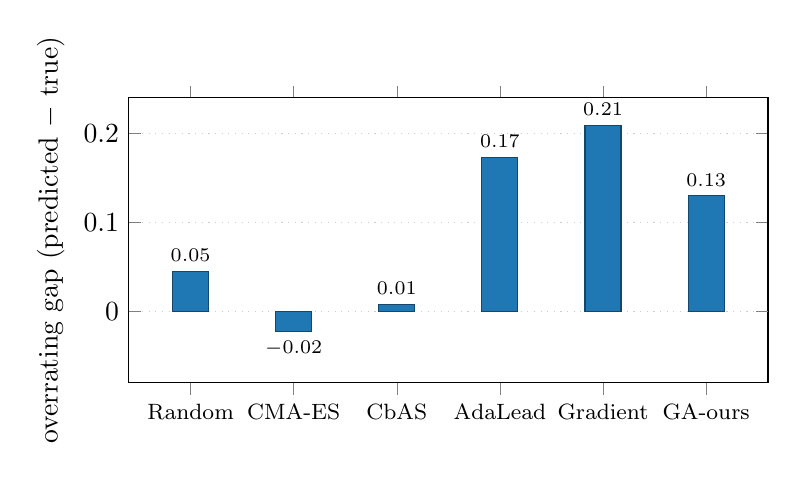
\begin{tikzpicture}
\begin{axis}[
  width=0.8\textwidth, height=5.2cm,
  ybar, bar width=13pt,
  ymin=-0.08, ymax=0.24,
  ylabel={overrating gap (predicted $-$ true)},
  symbolic x coords={Random, CMA-ES, CbAS, AdaLead, Gradient, GA-ours},
  xtick=data, x tick label style={font=\footnotesize},
  nodes near coords, every node near coord/.append style={font=\scriptsize,/pgf/number format/fixed,/pgf/number format/precision=2},
  ymajorgrids, major grid style={dotted,gray!40},
  extra y ticks={0}, extra y tick labels={}, extra y tick style={grid=major, grid style={solid,black!55}},
  enlarge x limits=0.12,
]
\addplot[fill=cOurs,draw=cOurs!60!black] coordinates
 {(Random,0.045) (CMA-ES,-0.022) (CbAS,0.008) (AdaLead,0.173) (Gradient,0.209) (GA-ours,0.130)};
\end{axis}
\end{tikzpicture}
\caption{\textbf{How much each method overrates its designs on TF-Bind-8 (5 seeds, same
query budget).} All methods reach $\approx0.89$ true score for their best designs, so they do
not separate on performance. They differ in how far the surrogate's predicted score sits
above the true score; gradient ascent and AdaLead overrate the most.}
\label{fig:tfbind}
\end{figure}

\subsection{The design system works: head-to-head on two protein tasks}

\paragraph{Thermostability (Meltome).}
All four methods reach a similar real gain ($+5.9$ to $+6.8\,^{\circ}$C, counting only the
starting points that were realistic to begin with). Where they differ is in how natural the
designs look (Figure~\ref{fig:meltome}, Table~\ref{tab:meltome}). Our biological rule gives
the most natural designs: it matches the learned second model (GABO; paired Wilcoxon
$p=0.36$, meaning no significant difference) and beats both the hand-tuned penalty (COMs) and
the unconstrained search ($p<0.001$).

\begin{table}[t]
\centering\small
\caption{Thermostability head-to-head ($n=40$ starting sequences; gain is counted over the
starting points that were realistic to begin with). The naturalness significance is a paired
Wilcoxon test, ours versus each baseline.}
\label{tab:meltome}
\begin{tabular}{lrrrl}
\toprule
Method & Real gain ($^{\circ}$C) & Naturalness $\Delta$PLL & Biophysical pass \% & vs.\ ours (naturalness) \\
\midrule
Unconstrained & $+6.8$ & $-0.191$ & 85 & $p<0.001$ \\
COMs          & $+6.5$ & $-0.206$ & 88 & $p<0.001$ \\
GABO/aSCR     & $+5.9$ & $-0.139$ & 85 & $p=0.36$ (n.s.) \\
\textbf{Ours} & $+6.3$ & $\mathbf{-0.128}$ & \textbf{90} & --- \\
\bottomrule
\end{tabular}
\end{table}

\begin{figure}[t]
\centering
\tikzsetnextfilename{meltome}
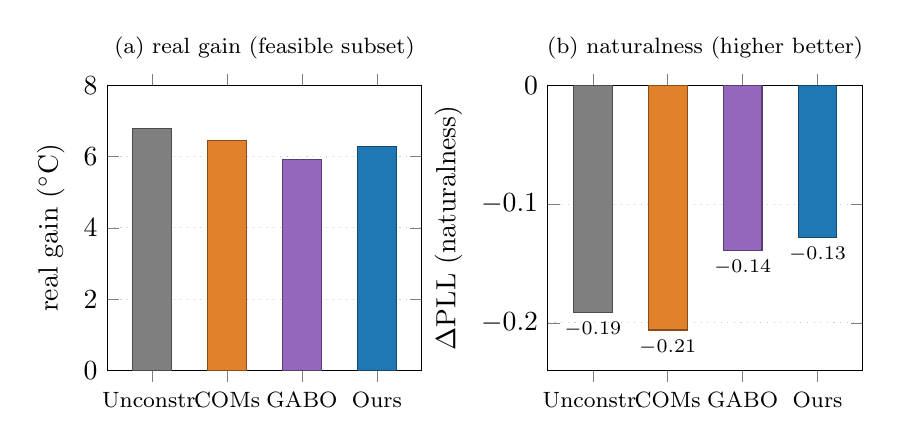
\begin{tikzpicture}
\begin{groupplot}[
  group style={group size=2 by 1, horizontal sep=1.6cm},
  width=0.46\textwidth, height=5.2cm,
  symbolic x coords={Unconstr., COMs, GABO, Ours},
  xtick={Unconstr., COMs, GABO, Ours}, x tick label style={font=\footnotesize},
  ymajorgrids, major grid style={dotted,gray!40}, ybar, /tikz/bar width=14pt, /tikz/bar shift=0pt,
  enlarge x limits=0.2,
]
\nextgroupplot[ylabel={real gain ($^{\circ}$C)}, ymin=0, ymax=8,
  title={\footnotesize (a) real gain (feasible subset)}]
\addplot[fill=cUnc,draw=cUnc!60!black] coordinates {(Unconstr.,6.79)};
\addplot[fill=cCOMs,draw=cCOMs!60!black] coordinates {(COMs,6.46)};
\addplot[fill=cGABO,draw=cGABO!60!black] coordinates {(GABO,5.93)};
\addplot[fill=cOurs,draw=cOurs!60!black] coordinates {(Ours,6.28)};
\nextgroupplot[ylabel={$\Delta$PLL (naturalness)}, ymin=-0.24, ymax=0,
  title={\footnotesize (b) naturalness (higher better)},
  nodes near coords, every node near coord/.append style={font=\scriptsize,/pgf/number format/fixed,/pgf/number format/precision=2}]
\addplot[fill=cUnc,draw=cUnc!60!black] coordinates {(Unconstr.,-0.191)};
\addplot[fill=cCOMs,draw=cCOMs!60!black] coordinates {(COMs,-0.206)};
\addplot[fill=cGABO,draw=cGABO!60!black] coordinates {(GABO,-0.139)};
\addplot[fill=cOurs,draw=cOurs!60!black] coordinates {(Ours,-0.128)};
\end{groupplot}
\end{tikzpicture}
\caption{\textbf{Thermostability head-to-head (Meltome, $n=40$).} (a) Real gains are similar
across methods. (b) Our rule gives the most natural designs, matching GABO and beating COMs
and the unconstrained search ($p<0.001$).}
\label{fig:meltome}
\end{figure}

\paragraph{Fluorescence (GFP).}
On GFP the difference is large (Figure~\ref{fig:gfp}). Our rule keeps 100\% of designs inside
the realistic biophysical range, versus 5\% (unconstrained), 11\% (COMs), and 19\% (GABO);
all three gaps are significant at $p<10^{-7}$. The predicted gain is a little lower for our
rule ($+0.71$ versus $+0.83$ to $+0.96$)---a small price for designs that are consistently
realistic.

\begin{figure}[t]
\centering
\tikzsetnextfilename{gfp}
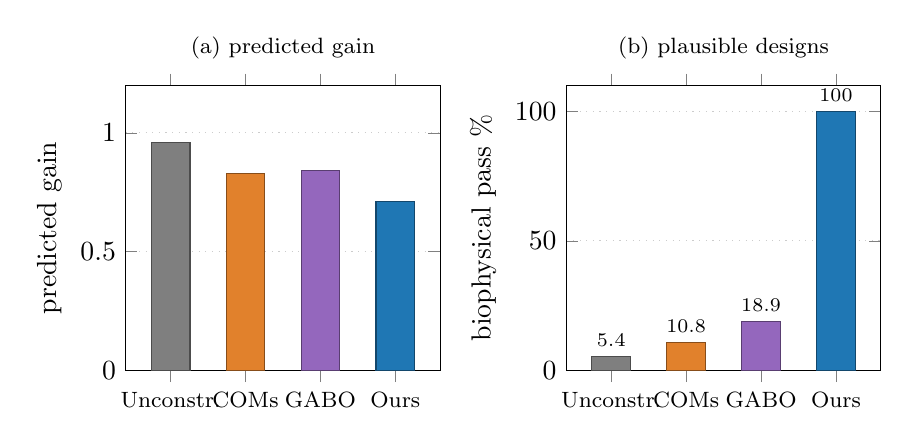
\begin{tikzpicture}
\begin{groupplot}[
  group style={group size=2 by 1, horizontal sep=1.6cm},
  width=0.46\textwidth, height=5.2cm,
  symbolic x coords={Unconstr., COMs, GABO, Ours},
  xtick={Unconstr., COMs, GABO, Ours}, x tick label style={font=\footnotesize},
  ymajorgrids, major grid style={dotted,gray!40}, ybar, /tikz/bar width=14pt, /tikz/bar shift=0pt,
  enlarge x limits=0.2,
]
\nextgroupplot[ylabel={predicted gain}, ymin=0, ymax=1.2,
  title={\footnotesize (a) predicted gain}]
\addplot[fill=cUnc,draw=cUnc!60!black] coordinates {(Unconstr.,0.96)};
\addplot[fill=cCOMs,draw=cCOMs!60!black] coordinates {(COMs,0.83)};
\addplot[fill=cGABO,draw=cGABO!60!black] coordinates {(GABO,0.84)};
\addplot[fill=cOurs,draw=cOurs!60!black] coordinates {(Ours,0.71)};
\nextgroupplot[ylabel={biophysical pass \%}, ymin=0, ymax=110,
  title={\footnotesize (b) plausible designs},
  nodes near coords, every node near coord/.append style={font=\scriptsize}]
\addplot[fill=cUnc,draw=cUnc!60!black] coordinates {(Unconstr.,5.4)};
\addplot[fill=cCOMs,draw=cCOMs!60!black] coordinates {(COMs,10.8)};
\addplot[fill=cGABO,draw=cGABO!60!black] coordinates {(GABO,18.9)};
\addplot[fill=cOurs,draw=cOurs!60!black] coordinates {(Ours,100)};
\end{groupplot}
\end{tikzpicture}
\caption{\textbf{Fluorescence head-to-head (GFP, $n=37$ realistic starting points).}
(a) Predicted gains are similar. (b) Fraction of designs inside the realistic biophysical
range: 100\% for our rule versus 5--19\% for the baselines (all $p<10^{-7}$).}
\label{fig:gfp}
\end{figure}

\subsection{The system generalizes to a third modality: regulatory DNA}

To test that the system is not specific to proteins, we applied it to a very different
molecule type: designing 600-base-pair regulatory DNA for higher chromatin accessibility.
Here the featurization is a frozen Evo2 genomic embedding, the biological rule is the
DNA composition band, and the true property is read out by Borzoi
\citep{linder2025borzoi}---a published model of DNA activity that the search never queried,
serving as the independent oracle. Running the same search loop used for the protein tasks,
the system raised the true Borzoi-measured accessibility on \textbf{all 40 of 40 starting
points} (mean rising from $0.09$ to $0.21$--$0.29$ in oracle units). The design engine and
the biological rule therefore transfer intact from protein to DNA.

This task also gives a clean second look at the surrogate ablation. At 600 base pairs the
genomic foundation model finally decodes the property competitively (held-out $\rho=0.73$,
against $0.70$ for a plain $k$-mer encoding)---a reversal of the short-DNA result in
Table~\ref{tab:decode}. Yet in \emph{design} the foundation-model surrogate does not beat the
plain encoding: the true gains are statistically indistinguishable ($+0.20$ for both,
unconstrained, paired Wilcoxon $p=0.48$; $+0.12$ versus $+0.16$ constrained, $p=0.22$). The
foundation model's higher \emph{predicted} gain does not convert to a higher \emph{true}
gain---the excess is surrogate overrating, exactly the effect the constrained loop and the
true oracle are built to catch. This reinforces the ablation's message: the surrogate is a
swappable component, and the system's power does not come from it.

\subsection{Independent validation}

The load-bearing part of the system is that no design claim rests on the surrogate grading
its own work: every task is confirmed by a signal the search never used. Across the four
tasks these signals are a held-out predictor ensemble, a separate model family (TemStaPro),
a structure predictor (AlphaFold2), the known GFP functional residues, an exact ground-truth
oracle (TF-Bind-8), and a true DNA-activity model (Borzoi). This protocol---not a new
optimizer---is the methodological contribution. The protein-task details follow
(Table~\ref{tab:validation}). On thermostability, a separate predictor (TemStaPro) and
AlphaFold2 both rank our designs as the most realistic. On GFP, our designs keep all five
known important residues intact in 87.5\% of cases, versus 67.5--77.5\% for the baselines,
and keep the key position Ser65 intact every time; the surrogate was never told these
positions matter. AlphaFold2 shows that every method still folds into a valid structure
(all 10 designs score pLDDT $\ge 70$), and our designs change the structure the least
($\Delta$pLDDT $-0.6$, versus $-1.2$ to $-1.5$ for the others).

\begin{table}[t]
\centering\small
\caption{Surrogate-blind validation. GFP functional-residue preservation is over $n=40$
designs; AlphaFold2 $\Delta$pLDDT is over a subset of $n=10$ (Meltome and GFP each).}
\label{tab:validation}
\begin{tabular}{lrrrr}
\toprule
Measure & Unconstrained & COMs & GABO/aSCR & Ours \\
\midrule
GFP: all 5 functional residues intact (\%) & 70.0 & 67.5 & 77.5 & \textbf{87.5} \\
GFP: Ser65 preserved (\%) & 82.5 & 87.5 & 87.5 & \textbf{100.0} \\
GFP: AlphaFold2 $\Delta$pLDDT vs.\ start & $-1.45$ & $-1.26$ & $-1.22$ & $\mathbf{-0.64}$ \\
\bottomrule
\end{tabular}
\end{table}

\subsection{When the rule helps, and when it hurts}

The constraint improves naturalness on Meltome and the biophysical pass rate on GFP. This
difference has a simple cause: how narrow the range of realistic sequences is
(Figure~\ref{fig:feasible}). GFP is a single 238-residue protein, so its biophysical range
is 8--19 times narrower than Meltome's, which spans thousands of distinct proteins. When the
range is
narrow, random changes leave it quickly (after 26 edits, only 3\% of GFP designs are still
in range, versus 99\% for Meltome), so the biophysical check is the one doing the work. When
the range is wide, most candidates pass it, so the biophysical check no longer separates
methods and the naturalness of the design does instead. In short, the constraint helps
through whichever check is hard to pass, and which check that is depends on how many
distinct proteins the training data covers: one protein gives a narrow range, thousands
give a wide one.

\paragraph{When the rule hurts: the range must match the true objective.}
The rule is not free. It only helps when the realistic range it enforces actually contains
the genuinely good sequences---when the range is \emph{aligned} with the true objective. If
the range excludes good sequences, the rule raises the pass rate while lowering the true
property: it looks like compliance but is really the constraint fighting the objective. We
see this on a DNA binding task (WT1), whose true binding motif is a run of cytosines. The
generic composition band caps repeated letters, so it rejects most of the strongest true
binders; the rule then reports 100\% ``realistic'' designs while the true binding drops. The
practical lesson, which we followed for the regulatory-DNA task above, is to derive the
range from the training distribution of the actual task rather than from a generic rule, so
that the range and the objective agree.

\begin{figure}[t]
\centering
\tikzsetnextfilename{feasible}
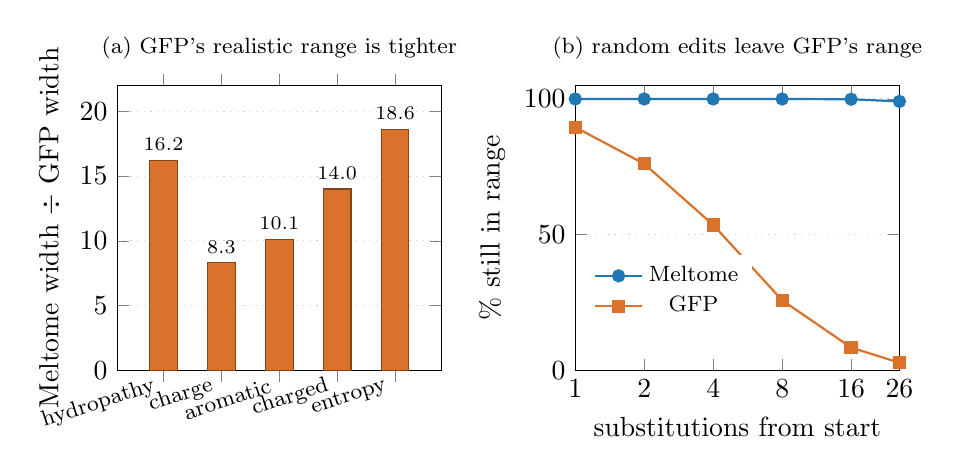
\begin{tikzpicture}
\begin{groupplot}[
  group style={group size=2 by 1, horizontal sep=1.7cm},
  width=0.47\textwidth, height=5.2cm,
  ymajorgrids, major grid style={dotted,gray!40},
]
\nextgroupplot[ybar, bar width=10pt, ymin=0, ymax=22,
  ylabel={Meltome width $\div$ GFP width},
  symbolic x coords={hydropathy, charge, aromatic, charged, entropy},
  xtick=data, x tick label style={rotate=18,anchor=east,font=\footnotesize},
  enlarge x limits=0.2,
  title={\footnotesize (a) GFP's realistic range is tighter},
  nodes near coords, every node near coord/.append style={font=\scriptsize,/pgf/number format/fixed,/pgf/number format/fixed zerofill,/pgf/number format/precision=1}]
\addplot[fill=cGFP,draw=cGFP!60!black,bar shift=0pt] coordinates
 {(hydropathy,16.2) (charge,8.3) (aromatic,10.1) (charged,14.0) (entropy,18.6)};
\nextgroupplot[ymin=0, ymax=105, xmin=1, xmax=26,
  xlabel={substitutions from start}, ylabel={\% still in range},
  title={\footnotesize (b) random edits leave GFP's range},
  legend style={at={(0.03,0.15)},anchor=south west,font=\footnotesize,draw=none},
  xmode=log, log basis x=2, xtick={1,2,4,8,16,26}, xticklabels={1,2,4,8,16,26},
  mark size=2pt]
\addplot[color=cOurs,mark=*,thick] coordinates
 {(1,100)(2,100)(4,100)(8,100)(16,99.9)(26,99.1)};
\addplot[color=cGFP,mark=square*,thick] coordinates
 {(1,89.6)(2,76.1)(4,53.6)(8,25.8)(16,8.4)(26,2.8)};
\legend{Meltome, GFP}
\end{groupplot}
\end{tikzpicture}
\caption{\textbf{Why the constraint helps through a different check on each task.}
(a) GFP's range of realistic sequences is 8--19$\times$ narrower than Meltome's on every
biophysical descriptor, because GFP is one protein and Meltome is thousands. (b) Random
substitutions leave GFP's narrow range quickly but stay inside Meltome's wide one, so the
biophysical check is the hard one for GFP and naturalness is the hard one for Meltome.}
\label{fig:feasible}
\end{figure}

\section{Related work}

Designing sequences by maximizing a learned surrogate, and the tendency of that search to
find the surrogate's mistakes, are both well studied
\citep{trabucco2021coms, trabucco2022designbench, fu2021nemo}. Known fixes include the
hand-tuned penalty \citep{trabucco2021coms}, a learned second model that scores how
training-like a sequence is \citep{yao2024gabo}, and biological priors built into the way
sequences are sampled \citep{prospero2025}. Recent work measures how these surrogates fail
on biological sequences \citep{overconfident2025} and reports that the failure does not
happen in every setting \citep{yang2025taco}. Foundation-model sequence design is also
advancing for DNA and RNA \citep{zhang2026aptamer, wang2024aptadiff}; those methods
keep training the language model further and search in a learned internal space, whereas we
keep the model frozen and search directly over sequences. Finally, genomic foundation models
are known to be foolable when used as classifiers
\citep{yoo2024dnalm, luo2025genoarmory, safegenes2025, krishnan2026adversarial}---the
same weakness our search exploits and our validation guards against. In our own earlier work
we used exactly this attack---a black-box genetic search over sequences---to show that
adversarial genomic sequences can evade biosecurity screening \citep{krishnan2026adversarial};
here we turn the same engine around and ask what it takes to make it \emph{design} rather
than merely fool. Our contribution is not a new optimizer but a
\emph{system}: reusing attack-style search as a design engine, a training-free biological
rule that keeps it realistic as well as a learned second model does, a surrogate-blind
validation protocol demonstrated across four tasks and two molecule types, and a
characterization of when the rule helps and when a misaligned rule hurts.

\section{Limitations}

All our tests are computational; testing designs in the lab is future work, and our
independent checks are themselves models, though the TF-Bind-8 oracle is an exact
ground-truth lookup. The biophysical
check looks at whole-sequence numbers and may miss structural details, which is partly why
we also run AlphaFold2 and the important-residue check. Our most expensive checks use small
samples ($n=10$--$16$), though the main design and plausibility results use all 40 starting
points per task. The search machinery is assembled from known pieces; the contribution is
the validated, characterized system, not a new optimizer. Finally, as the mechanism section
shows, the rule helps only when its range is tight and aligned with the true objective---a
misaligned range can be cosmetic or even counterproductive, so the range must be built from
the task's own training distribution.

\section{Conclusion}

The search that produces adversarial examples can be turned into a biological sequence
designer by adding two things: a training-free biological rule that keeps the search
realistic, and a validation protocol that confirms every design against signals the search
never used. The rule matches a learned second model and beats a hand-tuned penalty, at a
similar predicted gain and without training anything extra. The system raises the true
property on three design tasks spanning proteins and DNA---confirmed on every task by an
independent signal, including an exact oracle and a true DNA-activity model---and we
characterize when the rule helps and when a misaligned rule hurts. Which featurization the
surrogate uses is a swappable component that changes none of these claims.

\small
\bibliographystyle{plainnat}
\bibliography{refs}
\end{document}
